\documentclass[cjk,xcolor=dvipsnames,envcountsect,notheorems,12pt]{beamer}
% * 16:9 のスライドを作るときは、aspectratio=169 を documentclass のオプションに追加する
% * 印刷用の配布資料を作るときは handout を documentclass のオプションに追加する
%   (overlay が全て一つのスライドに出力される)

\graphicspath{ {./images/} }
\hypersetup{unicode=true}% しおりの文字化け対策
\usepackage[no-math]{fontspec}
\usepackage{luatexja,luatexja-fontspec}
\usepackage{amsmath,amssymb,amsfonts,amsthm,ascmac,cases,bm,pifont}
\usepackage{graphicx}
\usepackage{url}

% スライドのテーマ
\usetheme{sumiilab}
% ベースになる色を指定できる
%\usecolortheme[named=Magenta]{structure}
% 数式の文字が細くて見難い時は serif の代わりに bold にしましょう
%\mathversion{bold}

% フォントの設定
\setmainfont[Ligatures=TeX]{TeXGyreTermes}
\setsansfont[Ligatures=TeX]{TeXGyreHeros}
\setmainjfont{RictyDiminished}
\setsansjfont{RictyDiminished}
%\setmainjfont[BoldFont=RictyDiminished-Bold]{RictyDiminished-Regular}

%% ===============================================
%% スライドの表紙および PDF に表示される情報
%% ===============================================

%% 発表会の名前とか(省略可)
\session{研究室ゼミ}
%% スライドのタイトル
\title{住井研究室の\\ステキな Beamer テンプレート}
%% 必要ならば、サブタイトルも
%\subtitle{}
%% 発表者のお名前
\author{ラムダ 小太郎}
%% 発表者の所属([] 内は短い名前)
%\institute[東北大学 住井・松田研]{東北大学 工学部 電気情報物理工学科\\住井・松田研究室}% 学部生
\institute[東北大学 住井・松田研]{東北大学 大学院 情報科学研究科\\住井・松田研究室}% 院生
%% 発表する日
\date{2000年1月1日}

%% ===============================================
%% 自動挿入される目次ページの設定(削除しても可)
%% ===============================================

%% section の先頭に自動挿入される目次ページ(削除すると、表示されなくなる)
\AtBeginSection[]{
\begin{frame}
  \frametitle{アウトライン}
  \tableofcontents[sectionstyle=show/shaded,subsectionstyle=show/show/hide]
\end{frame}}
%% subsection の先頭に自動挿入される目次ページ(削除すると、表示されなくなる)
\AtBeginSubsection[]{
\begin{frame}
  \frametitle{アウトライン}
  \tableofcontents[sectionstyle=show/shaded,subsectionstyle=show/shaded/hide]
\end{frame}}

%% 現在の section 以外を非表示にする場合は以下のようにする

%% \AtBeginSection[]{
%% \begin{frame}
%%   \frametitle{アウトライン}
%%   \tableofcontents[sectionstyle=show/hide,subsectionstyle=show/show/hide]
%% \end{frame}}
%% \AtBeginSubsection[]{
%% \begin{frame}
%%   \frametitle{アウトライン}
%%   \tableofcontents[sectionstyle=show/hide,subsectionstyle=show/shaded/hide]
%% \end{frame}}

%% ===============================================
%% 定理環境の設定
%% ===============================================

\setbeamertemplate{theorems}[numbered]% 定理環境に番号を付ける
\theoremstyle{definition}
\newtheorem{definition}{定義}
\newtheorem{axiom}{公理}
\newtheorem{theorem}{定理}
\newtheorem{lemma}{補題}
\newtheorem{corollary}{系}
\newtheorem{proposition}{命題}

%% ===============================================
%% ソースコードの設定
%% ===============================================

\usepackage{listings,jlisting}
%\usepackage[scale=0.9]{DejaVuSansMono}

\definecolor{DarkGreen}{rgb}{0,0.5,0}
% プログラミング言語と表示するフォント等の設定
\lstset{
  language={[Objective]Caml},% プログラミング言語
  basicstyle={\ttfamily\small},% ソースコードのテキストのスタイル
  keywordstyle={\bfseries},% 予約語等のキーワードのスタイル
  commentstyle={},% コメントのスタイル
  stringstyle={},% 文字列のスタイル
  frame=trlb,% ソースコードの枠線の設定 (none だと非表示)
  numbers=none,% 行番号の表示 (left だと左に表示)
  numberstyle={},% 行番号のスタイル
  xleftmargin=5pt,% 左余白
  xrightmargin=5pt,% 右余白
  keepspaces=true,% 空白を表示する
  mathescape,% $ で囲った部分を数式として表示する ($ がソースコード中で使えなくなるので注意)
  % 手動強調表示の設定
  moredelim=[is][\itshape]{@/}{/@},
  moredelim=[is][\color{red}]{@r\{}{\}@},
  moredelim=[is][\color{blue}]{@b\{}{\}@},
  moredelim=[is][\color{DarkGreen}]{@g\{}{\}@},
}

%% ===============================================
%% 本文
%% ===============================================
\begin{document}
\frame[plain]{\titlepage}% タイトルページ

\section*{アウトライン}

% 目次を表示させる(section を表示し、subsection は隠す)
\begin{frame}
  \frametitle{アウトライン}
  \tableofcontents[sectionstyle=show,subsectionstyle=hide]
\end{frame}

\section{単純な使い方}

\subsection{フォント}

% * \begin{frame} と \end{frame} で囲った部分にスライドの内容を書く
% * \frametitle{...} にスライドのタイトルを書く
\begin{frame}
  \frametitle{フォント}
  {\scriptsize こんにちは、世界。}\\
  {\footnotesize こんにちは、世界。}\\
  {\small こんにちは、世界。}\\
  こんにちは、世界。\\% {\normalsize こんにちは、世界。}
  {\large こんにちは、世界。}\\
  {\Large こんにちは、世界。}\\
  {\LARGE こんにちは、世界。}\\
  {\Huge こんにちは、世界。}
  \vfill% 縦方向によく伸びる空白(適当に間隔を開けたい時に便利)
  \structure{こんにちは、世界。}\\% 強調表示1
  \alert{こんにちは、世界。}% 強調表示2
\end{frame}

\subsection{箇条書き}

\begin{frame}
  \frametitle{箇条書き}
  番号なし箇条書き:
  \begin{itemize}
  \item 項目1
  \item 項目2
  \item 項目3
  \end{itemize}
  番号つき箇条書き:
  \begin{enumerate}
  \item 項目1
  \item 項目2
  \item 項目3
  \end{enumerate}
\end{frame}

\section{ちょっと特殊な機能}

\subsection{ブロック}

\begin{frame}
  \frametitle{ブロックの使用例}
  \begin{block}{ブロックのタイトル}
    ブロックの内容。
  \end{block}
  \vfill
  \begin{exampleblock}{ブロックのタイトル}
    exampleblock は例のためのブロックです。
  \end{exampleblock}
  \vfill
  \begin{alertblock}{ブロックのタイトル}
    alertblock は強調のためのブロックです。
    alert のブロック版だと思えばいいでしょう。
  \end{alertblock}
\end{frame}

\begin{frame}
  \frametitle{定理環境の使用例}
  \renewcommand{\thedefinition}{1.1}% 定義の番号
  \begin{definition}[定義のタイトル]
    定義の内容
  \end{definition}
  \vfill
  \renewcommand{\thelemma}{2.2}% 補題の番号
  \begin{lemma}[補題のタイトル]
    補題の内容
  \end{lemma}
  \vfill
  \renewcommand{\thetheorem}{3.4}% 定理の番号
  \begin{theorem}[定理のタイトル]
    定理の内容
  \end{theorem}
  \vfill
  \begin{proof}[証明のタイトル]
    証明の内容
  \end{proof}
\end{frame}

\begin{frame}
  \frametitle{ブロック環境}
  次の環境が使えます。
  \begin{itemize}
  \item block
  \item exampleblock
  \item alertblock
  \item 定義(definition)
  \item 公理(axiom)
  \item 定理(theorem)
  \item 補題(lemma)
  \item 系(corollary)
  \item 命題(proposition)
  \item 証明(proof) --- 他の環境と少しだけ使い方が違うので注意
  \end{itemize}
  ※ block, exampleblock, alertblock はただの色違い。それ以外は block 環境と同じ色。
\end{frame}

\subsection{オーバーレイ}

\begin{frame}
  \frametitle{オーバーレイ}
  \alert{オーバーレイ(overlay)}とは、
  \begin{itemize}
    \pause% \pause 以降の文章は後から表示される
    \item 単純なアニメーションみたいなもの
    \pause
    \item 最初のスライドでは隠していた文字や図形を、あとから表示させる
    \pause
    \item よく使うのは pause(他にもいろいろある)
  \end{itemize}
\end{frame}

\section{ソースコードの書き方}

\begin{frame}
  \frametitle{ソースコードの書き方}
  ソースコードは verbatim 環境でも書けるが、あまり綺麗ではない。
  \vfill
  listings を使うのがおすすめ :
  \begin{itemize}
  \item listings.sty --- LaTeX で綺麗なソースコードを書くためのスタイルファイル
  \item jlisting.sty --- ソースコード中で日本語を使いたい時に必要(listings.sty と併用)
  \end{itemize}
\end{frame}

\begin{frame}
  \renewcommand{\baselinestretch}{1.3}% 箇条書き項目の間隔を広げる (詰まり過ぎると見難いので)
  \frametitle{ソースコードの書き方}
  \begin{itemize}
  \item frame 環境のオプションに fragile を指定する
    \begin{itemize}
    \item 指定の方法はソースコードを参照
    \item 指定しないと、コンパイルできない
    \end{itemize}
  \item listings はあまり高度な自動色付けができない
    \begin{itemize}
    \item せいぜい、予約語の強調とか、文字列・コメントの色つけ程度
    \item 細かい強調は手動で行ったほうが良い(後述)
    \end{itemize}
  \end{itemize}
\end{frame}

\begin{frame}[fragile]% frame 環境のオプションに fragile を指定
  \frametitle{ソースコードの例}
  \begin{itemize}
  \item 長いソースコードには lstlisting 環境を使う
  \item 文中のソースコードには lstinline マクロを使う(用法は verb と同じ)
  \end{itemize}
  \vfill
  例1) lstlisting 環境:
\begin{lstlisting}
type 'a bin_tree =
  | Leaf of 'a
  | Node of 'a bin_tree * 'a bin_tree

let rec listup_nodes = function
  | Leaf x -> [x]
  | Node (r, l) -> (listup_nodes r) @ (listup_nodes l)
\end{lstlisting}
  \vfill
  例2) lstinline マクロ:\\
  \lstinline|listup_nodes| の型は \lstinline|'a bin_tree -> 'a list| である。
\end{frame}

\subsection{一時的にスタイル or 言語を変更する}

\begin{frame}[fragile]% frame 環境のオプションに fragile を指定
  \frametitle{一時的にスタイル or 言語を変更する}
  ソースコードの強調表示の設定:
  \begin{itemize}
  \item 共通の定義はプリアンブルの lstset で行う。
  \item 個別に変更するときは、lstlisting、lstinline のオプションで指定する。
  \end{itemize}
  \vfill
  例1) フレームなし
\begin{lstlisting}[frame=none]
let rec fact n =
  if n = 0 then 1 else n * (fact (n - 1))
\end{lstlisting}
  \vfill
  例2) C 言語に変更
\begin{lstlisting}[language=C]
int fact (int n) {
  if (n == 0) {
    return 1;
  } else {
    return n * fact(n - 1);
  }
}
\end{lstlisting}
\end{frame}

\subsection{ソースコードの手動強調表示}

\begin{frame}[fragile]% frame 環境のオプションに fragile を指定
  \frametitle{ソースコードの手動強調表示}
  以下の書式で強調表示ができるようになっている。\\
  (使い方はソースコードを参照)
  \begin{itemize}
  \item \verb|@/.../@| --- イタリック:\lstinline|@/hoge/@|
  \item \verb|@r{...}@| --- 赤:\lstinline|@r{hoge}@|
  \item \verb|@g{...}@| --- 緑:\lstinline|@g{hoge}@|
  \item \verb|@b{...}@| --- 青:\lstinline|@b{hoge}@|
  \end{itemize}
  \vfill
  例)
\begin{lstlisting}
let fact n
  let rec @g{fact'}@ @b{i}@ @r{acc}@ =
    if @b{i = 0}@ then @r{acc}@ else @g{fact'}@ @b{(i - 1)}@ @r{(n * acc)}@
  in
  @g{fact'}@ @b{n}@ @r{1}@
\end{lstlisting}
\end{frame}

\section{レイアウト}

\begin{frame}
  \frametitle{columns/column 環境}
  \begin{columns}%% columns 環境の中に column 環境を入れる
    \begin{column}{0.2\textwidth}%% [横幅] 0.2\textwidth = ページ幅の 20 %
      %% ページの左側に表示される内容:
      \begin{center}
        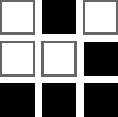
\includegraphics{sample-image.pdf}
      \end{center}
    \end{column}
    \begin{column}{0.8\textwidth}
      %% ページの右側に表示される内容:
      \begin{itemize}
      \item ページを横に分割
      \item 図・表・文を横に並べて配置可能
      \item よく使うレイアウト
      \item minipage 環境でも同じ事ができる
      \end{itemize}
    \end{column}
  \end{columns}
  \pause\vfill
  \begin{columns}%% columns 環境の中に column 環境を入れる
    \begin{column}{0.4\textwidth}
      %% ページの左側に表示される内容:
      \begin{center}
        入れ子にしてみる
      \end{center}
      \begin{columns}
        \begin{column}{0.33\textwidth}
          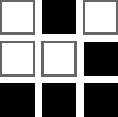
\includegraphics[width=\textwidth]{sample-image.pdf}
        \end{column}
        \begin{column}{0.33\textwidth}
          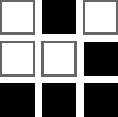
\includegraphics[width=\textwidth]{sample-image.pdf}
        \end{column}
        \begin{column}{0.33\textwidth}
          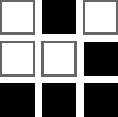
\includegraphics[width=\textwidth]{sample-image.pdf}
        \end{column}
      \end{columns}
    \end{column}
    \begin{column}{0.6\textwidth}
      %% ページの右側に表示される内容:
      \begin{itemize}
      \item 3 つ以上の分割も可能
      \item 入れ子も可能
      \item 柔軟に使えて便利!
      \end{itemize}
    \end{column}
  \end{columns}
\end{frame}

%% ===============================================
%% 予備スライド
%% ===============================================

%% 予備スライドは appendix 環境の中に書きましょう。
\begin{appendix}

%% 予備スライドの先頭に APPENDIX と書かれたページを挟む(お好みで消去しても良い)
\frame[plain]{\centerline{\Huge\bfseries\color{structure}APPENDIX}}

\section{予備のスライド}

\begin{frame}
  \frametitle{予備のスライド}
  予備スライドは appendix 環境の中に書きましょう。
\end{frame}

\end{appendix}

\end{document}
